%#!luajitlatex
\IfFileExists{luatex85.sty}{\RequirePackage{luatex85}}{}
\documentclass{ltjsarticle}

\usepackage{showexpl}
\lstset{pos=l, width=.4\textwidth,
  explpreset={numbers=left,numberstyle=\tiny,literate={\\\\}{}0 }}
% showexplの出力が邪魔なので表示しない
\makeatletter
\let\SX@Info=\relax
\makeatother

% TikZ, TikZ-cd
\usepackage{tikz}
\usetikzlibrary{patterns,cd}

%%% prettyref
\usepackage{prettyref}
\makeatletter
  \newrefformat{ex}{課題\nobreak\ref{#1}}
  \newrefformat{sec}{\S\ref{#1}}
  \newrefformat{ssec}{\S\ref{#1}}
  \newrefformat{fig}{図\nobreak\ref{#1}}
\makeatother

%%% fancyvrb
% \VerbatimFootnotes は \begin{document} の後で実行する
\usepackage{fancyvrb}

%%% \paragraph{} で「■課題 xx」という見出しをつける
%%% このような使い方は行儀が悪いのだが……
\makeatletter
\newcount\assignment@count
\assignment@count=1
\let\orig@paragraph=\paragraph
\def\paragraph#1{%
  \orig@paragraph{課題\the\assignment@count}\leavevmode%
  \global\advance\assignment@count1
  \protected\edef\@currentlabel{\the\assignment@count}\relax
}
\makeatother

% 更新日時の印字に datetime2 パッケージの \DTMnow を使う
% ただし, datetime2 パッケージは \today を上書きしようとするので,防止する
% また,タイムゾーンは印字しない
\let\origtoday=\today
\usepackage[datesep={/},timesep={:}]{datetime2}
\renewcommand\DTMdisplayzone[2]{}
\let\today=\origtoday

\usepackage{mystyle}
\hypersetup{pdftitle={TeX 実習}}
\title{\TeX 実習}
\date{\today}
\author{}

\begin{document}
\VerbatimFootnotes
\baselineskip1.75\zw
\maketitle

本文章は,\TeX 実習の実際の中身である.
行うためには実習用マシンに\TeX システムをインストールする必要がある.
計算数学実習資料集の
「\href{https://github.com/utmsks/KSImaterial/blob/master/contents/tex/tex_practice.md}{\TeX 実習}」
のページ内にある「\TeX~Liveのインストール」を参照すること.


\TeX~Liveをインストールした後は,各自の知識に沿って実習を進めてほしい,
\begin{itemize}
\item 今まで\TeX を全く触ったことがない人は\prettyref{sec:primer}へ.
\item 「\TeX・\LaTeX の典型的な間違い」については\prettyref{sec:typeset}へ.
\item \prettyref{sec:primer}や\prettyref{sec:typeset}を読んだら,
 それについての演習が\prettyref{sec:kadai}にあるので取り組んで欲しい.
% \item 日本語で\TeX 環境を書く際の文字コードに関する注意や,u\pTeX の話題は\prettyref{sec:chrcode}へ.
\item 各種パッケージを有効活用して相互参照,画像挿入,可換図式を組む方法については\prettyref{sec:ref}へ.
\item 伝統的な\pLaTeX は知っているが,\pLaTeX が利用できない場合への対処法や,
 最近の\TeX の発展について知りたい人は\prettyref{sec:other-engines}(執筆中)か,
 実習資料集にある「\pTeX 系列以外による日本語文書作成」(やや古い)を参照すること.
\item バリバリ使いこなしていて,以上の範囲などとっくに知っているという人はTAを呼ぶこと.
\end{itemize}

以下,\url{about:blank}のような部分は外部リンクで,緑字の部分
\footnote{Webブラウザ上では動作しないが,SumatraPDF などの PDF リーダーであれば動作する.}
は文書内リンクである.

\bigskip

\emph{\TeX ソース等の表記では,以下の字体(Inconsolata)を使っている}:
\begin{center}
\begin{tabular}{ccccc}
\toprule
数字の0&大文字のオー&数字の1&小文字のエル&大文字のアイ\\
\cmidrule(lr){1-2}\cmidrule(lr){3-5}
\Large\texttt{0}&\Large\texttt{O}
&\Large\texttt{1}&\Large\texttt{l}&\Large\texttt{I}\\
\bottomrule
\end{tabular}
\end{center}

\vfill

{\scriptsize\raggedleft
Last update: \texttt{\DTMnow}.
\par}

\newpage
\tableofcontents

\newpage
\section{\pLaTeX はじめの一歩}\label{sec:primer}
日本人が「\TeX を用いて文書を書く」という場合,実際に使っているのは
\emph{\pLaTeX}であることが多い.これらは,
\begin{itemize}
\item Knuth氏による,もともとの(プログラムとしての)\TeX
\item Leslie Lamport氏による,\href{http://www.latex-project.org/}%
  {\emph{\LaTeX}}という\TeX のマクロパッケージ
\end{itemize}
を,アスキー\footnote{当時.現在は株式会社KADOKAWA内の
アスキー・メディアワークス ブランドカンパニー.}が
それぞれ日本語化したものである.
細かく言うと,プログラム側は\pTeX\ (publishing \TeX)と呼ばれ,
\LaTeX を日本語対応させたマクロパッケージが\pLaTeX である% \footnote{%
%   どちらも公式ページは\url{http://ascii.asciimw.jp/pb/ptex/}であるが,
%   W32\TeX・\TeX~Live中の\pTeX は公式のものにかなり手が加えられている.
% }
.日本語では横書きの他に縦書きも行われるが,
\pTeX・\pLaTeX は縦組みの組版もサポートしている.

この実習では,\pTeX/\pLaTeX{}をUnicode対応させた\upTeX/\upLaTeX{}を使用する.
\pTeX{}系以外の\TeX{}エンジンについては,後の方(\prettyref{sec:other-engines})で軽く触れる.

\subsection{最初の例}
\label{ssec:first}
まず適当なエディタを使い,次の内容を持った\FNAME{first.tex}を作る.
このような\TeX が理解できるようなテキストファイルを\emph{\TeX ソース}という.
\begin{lstlisting}[numbers=left,numberstyle=\tiny,xleftmargin=3\zw]
\documentclass[uplatex]{jsarticle}
\begin{document}
ようこそ,\TeX の世界へ!
\[
  \int_0^\infty e^{-x^2}\,dx = \frac{\sqrt{\pi}}{2}.
\]
ちょっとチェックしちゃった。
\end{document}
\end{lstlisting}
\begin{itemize}
\item \emph{大文字と小文字,
全角文字と半角文字は厳密に区別されるので,間違えないように注意.
特に,半角バックスラッシュ~\SYM\textbackslash}~から始まる文字列は\TeX では
何らかの命令として扱われる.
\item Windowsで作業をしている関係で,
実際に編集を行うテキストエディタでは,半角バックスラッシュは
半角円記号~\SYM{\char165}~のように
表示されることになるだろう.
\item 保存先はどこでもいいが,
  以降の説明では「ドキュメント」のところに保存したとする.
\item ファイルの文字コードはUTF-8で保存する\footnote{%
    Windows上の\upTeX{}には文字コード自動判別機能があるのでShift\_JISで保存しても動くかもしれないが,今の時代はUnicode (UTF-8)を使うのが自然だろう.%
  }.
\end{itemize}

\medskip

1行目が\FNAME{first.tex}で用いる\emph{クラスファイル}を指定している箇所であり,
このクラスファイルが文書全体の大まかなレイアウトを規定する.
ここでは,奥村晴彦氏による
\href{http://oku.edu.mie-u.ac.jp/~okumura/jsclasses/}{\pLaTeXe 新ドキュメントクラス}%
の一つである\PKG{jsarticle}クラスを利用する.

\newpage

\subsection{タイプセット}
\label{ssec:typeset}
次に「コマンド プロンプト」を起動し,
\begin{lstlisting}
C:\Users\...> #\underline{cd\ Documents}#
C:\Users\...\Documents> #\underline{uplatex\ first.tex}#
\end{lstlisting}
と入力\footnote{ここでも,半角バックスラッシュは実際の画面では半角円記号で表示されているは
ずである.}すると,
\begin{lstlisting}
This is e-upTeX, Version 3.14159265-p3.8.1-u1.23-180226-2.6 (utf8.uptex)
 (TeX Live 2018/W32TeX) (preloaded format=uplatex)
 restricted \write18 enabled.
entering extended mode
……(中略)……
Output written on first.dvi (1 page, 840 bytes).
Transcript written on first.log.
\end{lstlisting}
のようなメッセージが出て%
\footnote{最初に「\texttt{e-}」という奇妙な文字列が見えるが,
  それについてはあまり気にしなくてもよい.},
「ドキュメント」の中に\FNAME{first.dvi}という
中間形式のファイルが生成される.
このように\TeX ソースからDVIファイルを生成することは
\emph{タイプセット},または\emph{コンパイル}と呼ばれる.

\medskip

\TeX を用いて文書を作成する場合,「DVIファイルを表示して中身を確認する」ことが
伝統的であったが,最近では「DVIからPDFファイルを生成し,それを最終成果物とする」
ことが(個人では)多くなり,それに伴い
PDFファイルを中身の確認にも用いることが多くなってきた\footnote{%
完全にPDFファイルに移行した,というわけではない.
DVIからPostScriptファイルに変換し,
それを成果物とする,というのもよく行われている.}.

本実習においても,\DVIPDFMx というプログラムによって
\FNAME{first.dvi}からPDFファイル\FNAME{first.pdf}を生成させ,
それを表示するという方針をとることにする.コマンドプロンプト上で
\begin{lstlisting}
C:\Users\...\Documents> #\underline{dvipdfmx\ first.dvi}#
\end{lstlisting}
と入力すると,
\begin{lstlisting}
first.dvi -> first.pdf
[1]
13562 bytes written
\end{lstlisting}
というメッセージが出て,PDFファイル\FNAME{first.pdf}が
無事に生成される.

\medskip
2012年後半以降の\TeX システムならば,
% \href{http://blog.preining.info/software-projects/ptex2pdf/}{\FNAME{ptex2pdf}}
\FNAME{ptex2pdf}というプログラムを使うことで,
\pLaTeX によるタイプセットとその後の\DVIPDFMx の処理をまとめて
\begin{lstlisting}
C:\Users\...\Documents> #\underline{ptex2pdf\ -l\ -u\ first.tex}#
\end{lstlisting}
で行うことができる.

\begin{lstlisting}
> ptex2pdf -l -u -ot "-synctex=1 -kanji=utf8" -od "-p jisb5" hoge.tex
\end{lstlisting}
のようにオプションを指定すると,次の2行の代わりとなる.
\begin{lstlisting}
> uplatex -synctex=1 -kanji=utf8 hoge.tex
> dvipdfmx -p jisb5 hoge.dvi
\end{lstlisting}

\paragraph{}
\FNAME{first.tex}の3行目
「\hbox{\ltjsetparameter{xkanjiskip=0pt}%
  \verb*+ようこそ,\TeX の世界へ!+}」を
それぞれ次のようにする.2つはエラーが出るが,それは何故か?\hskip.5\zw
また,残りの1つはどのようになるか?

ただし,コピー・ペーストはせずに手入力をすること.
その際には括弧内のコメントに注意.

\begin{itemize}\ltjsetparameter{xkanjiskip=0pt}
\item {\catcode`¥=12\verb*+ようこそ,¥TeX の世界へ!+} ({\catcode`¥=12\verb*+¥TeX+}全て全角文字)
\item \verb*+ようこそ,\TeXの世界へ!+ (半角スペースを省略)
\item \verb*+ようこそ,\TEX の世界へ!+ (Eも大文字)
\end{itemize}




\subsection{エラーが起きたら}
タイプセット中に,エラーが発生することがある.
以下は典型的なエラーの例で,2行目の``\verb+\begin{document}+''を
``\verb+\Begin{document}+''と間違えたことによって発生したエラーである:
\begin{lstlisting}
! Undefined control sequence.
<recently read> \Begin

l.2 \Begin
          {document}
?
\end{lstlisting}
このようなエラーメッセージが表示されると入力待ち状態になっているので,
\begin{itemize}
\item ``\verb+x+''と入力するとタイプセットはここで終了する.その後,
  画面上のエラーメッセージを参照して\FNAME{first.tex}の内容を修正することになる.
\item 一部のエラーについては,``\verb+h+''と入力することで
  ヘルプが表示されることがある:
\begin{lstlisting}
! Undefined control sequence.
<recently read> \Begin

l.2 \Begin
          {document}
? #\underline{h}#
The control sequence at the end of the top line
of your error message was never \def'ed. If you have
misspelled it (e.g., `\hobx'), type `I' and the correct
spelling (e.g., `I\hbox'). Otherwise just continue,
and I'll forget about whatever was undefined.

?
\end{lstlisting}
この場合なら,メッセージに従って``\verb+I\begin+''と入力することでエラーを修正することができるが,
もちろん後からソースファイル\FNAME{first.tex}の側も直しておかなければならない.
\end{itemize}

\newpage
エラーメッセージの内容については,\TeX~Wiki中の
「\href{https://texwiki.texjp.org/?LaTeX\%20\%E3\%81\%AE\%E3\%82\%A8\%E3\%83\%A9\%E3\%83\%BC\%E3\%83\%A1\%E3\%83\%83\%E3\%82\%BB\%E3\%83\%BC\%E3\%82\%B8}%
{\LaTeX のエラーメッセージ}」や
「\href{https://texwiki.texjp.org/?TeX\%20\%E3\%81\%AE\%E3\%82\%A8\%E3\%83\%A9\%E3\%83\%BC\%E3\%83\%A1\%E3\%83\%83\%E3\%82\%BB\%E3\%83\%BC\%E3\%82\%B8}%
{\TeX のエラーメッセージ}」
を参照してほしい.大体は自分の\TeX ソース側にエラーがあることが多いが,
次のような事態が起こったときは話が別である.
\begin{itemize}
\item ``\verb+! This can't happen+''というエラーメッセージが出たとき.
\item \pLaTeX が「不正な処理」などが原因で\emph{強制終了}されたとき.
\end{itemize}
上のどちらかの症状が発生したときは
\pTeX のバグの可能性があるので,発生した元のソースをとっておくと共に,TAに連絡すること.

\subsection{日本語フォントの埋め込み}

\TeX~Liveのデフォルトでは,(u)\pLaTeX+\DVIPDFMx{}で作ったPDFファイルには,IPAexフォントが埋め込まれている\footnote{%
  \TeX~Live~2015までは,(u)\pLaTeX+\DVIPDFMx{}で作ったPDFファイルにはデフォルトではフォントが埋め込まれていなかった.
}.

デフォルトで埋め込まれるフォントを変更する方法も用意されている.
例えば,\TeX~Liveに同梱されているIPAフォント(\href{http://ipafont.ipa.go.jp/}{公式サイト})
をPDF内に埋め込みたければ,コマンドプロンプトにおいて,
\begin{lstlisting}
C:\Users\...> #\underline{kanji-config-updmap\ --user\ ipa}#
\end{lstlisting}
または
\begin{lstlisting}
C:\Users\...> #\underline{updmap\ --user\ --setoption\ jaEmbed\ ipa}#
\end{lstlisting}
を実行すればよい\footnote{%
当然ながら,「PDF内にフォントを埋め込む」場合には,フォントのライセンスによって
許されていることを確認しないといけない.}.
以降の\DVIPDFMx の実行で作られるPDFファイルには,日本語フォントとして
IPA明朝・IPAゴシックが埋め込まれることになる.

% TODO: --userじゃなくて--sysを使うべき?

\medskip
macOSに商用・高品質なヒラギノフォントが付属していることは有名である%
\footnote{「ヒラギノを買ったらMacがおまけについてきた」という有名なジョークがある.}.
このヒラギノフォントを\TeX{}で利用することもできるが,追加の手順が必要となる.
詳しくは\TeX~Wikiの\href{https://texwiki.texjp.org/?%E3%83%92%E3%83%A9%E3%82%AE%E3%83%8E%E3%83%95%E3%82%A9%E3%83%B3%E3%83%88}{「ヒラギノフォント」}を参照して欲しい\footnote{%
  macOSのバージョンによってフォントファイルの仕様が変わる場合があること,
  \TeX~Wikiの更新はボランティアによって行われていることから,
  \TeX~Wikiの記述が最新のmacOSに当てはまらなかったとしても怒らないで頂きたい.
}.

\medskip
なお,\FNAME{kanji-config-updmap}や\FNAME{updmap}に\texttt{--user}を指定した場合は
自分のユーザーアカウントに対してのみ設定を行う.システム全体で設定したい場合は,
\texttt{--user}の代わりに\texttt{--sys}を指定する.
フォント埋め込み等の設定は,ユーザーごとの設定の方がシステム全体の設定よりも優先度が高いため,
一旦ユーザーの設定が作成されたあとはシステム全体の設定は使用されなくなる.

\newpage
\subsection{この先は}
ひとまず\pLaTeX によって文書を作成する基本的な方法が身についたので,
後は\LaTeX の文法を勉強すればよい.

本文書では,書体の変更とか箇条書きの書き方とかそういう
基本的な\LaTeX の文法については解説しない.
代わりに,Web上で参照できる入門ページとして
\begin{itemize}
\item \href{https://texwiki.texjp.org/}{\TeX~Wiki}中の「\TeX 入門」
\item 教育用計算機システム自習教材「\href{https://hwb.ecc.u-tokyo.ac.jp/wp/}{はいぱーワークブック}」%
  中の「27.~\LaTeX」
\item 渡辺徹,「好き好き\LaTeXe 初級編」,2004.\\
\url{http://mytexpert.osdn.jp/index.php?%B9%A5%A4%AD%B9%A5%A4%ADLaTeX2e%2F%BD%E9%B5%E9%CA%D4}
% \item 吉永徹美氏の「\href{http://www.h4.dion.ne.jp/~latexcat/index.html}{SMALL \LaTeX\
%       LAB}」中の「\LaTeX 入門」 % リンク切れ
\end{itemize}
を挙げておく.その他参考となるページには,
\begin{itemize}
\item 上田氏の「\href{http://www.fugenji.org/~thomas/texlive-guide/}{\TeX~Live を使おう}」
\item 熊澤吉起氏の\href{http://www.biwako.shiga-u.ac.jp/sensei/kumazawa/index.html}{Webサ
      イト}中の「\href{http://www.biwako.shiga-u.ac.jp/sensei/kumazawa/tex.html}{\TeX}」に
      は多数のパッケージの使用例がある.
\item Scott Pakin, \textit{The Comprehensive \LaTeX\ Symbol List}.\\
\url{https://ctan.org/pkg/comprehensive}\\
\hfill またはコマンドプロンプトで\texttt{texdoc comprehensive}を実行して\texttt{symbols-a4.pdf}を開く
\end{itemize}
があり,\TeX~Wiki中の「国内リンク」からも多くのページが辿れる.

\TeX{} Liveがインストールされた手元のPCにもマニュアル類(多くの場合は英語)が入っている.
それらは,コマンドプロンプトで\texttt{texdoc $\langle \textit{パッケージ名}\rangle$}を実行することによって参照できる.
例えば,\texttt{texdoc}コマンドのマニュアルを参照したければ,\texttt{texdoc texdoc}を実行すれば良い.

\medskip

本格的に学習する際には,\emph{まとまった参考書を入手することを強くお勧め}する.
「はいぱーワークブック」の「27.12~参考文献」にいくつか本があげられているし,
\TeX~Wikiの「\TeX の本」にもたくさんの本が紹介されている.

しかし,\emph{当たり前のことだが,一番大事なのは自分の書く文章の中身である}.
文書の価値は,あくまでもその内容によって上からおさえられるので,
\TeX・\LaTeX を適切に使い読みやすく見栄えの良い文書を作ったとしても,
それは文書の価値を上げることにはならない.%
%\footnote{一方,悪い組版によって,
%不当に価値が低く見られる可能性は十分にあるのだが.}.

\newpage
\subsection{日々の作業の小技}

\subsubsection{Sync\TeX}
\label{ssec:synctex}
\TeX を作って長い文章を作成していると,PDFの表示画面から\TeX ソースの
該当箇所の編集画面へと,またはその逆のジャンプができると便利である.
そのための機能として,最近の\pTeX などには\href{http://itexmac.sourceforge.net/SyncTeX.html}{\emph{Sync\TeX}}%
という機能が備わっている.

\medskip
Sync\TeX の機能を実習用マシンで使うには,以下の設定を行う.
\begin{description}
 \item[\TeX 側の指定] \pLaTeX によるタイプセット時に\texttt{-synctex=1}オプションを指定する.
 \item[SumatraPDF側の設定] 「設定」→「オプション」と辿り,「逆順検索コマンドラインの設定」\footnote{%
    先に上記の「\TeX 側の設定」を行わないと表示されない.}
	    に次のように入力する\footnote{%
    実行ファイルの場所はインストール時の設定によっては違っているかもしれない.デスクトップにあるショートカットを右クリックして「プロパティ」を開くと確認できる.}.
\begin{lstlisting}
"C:\Program Files\EmEditor\Emeditor.exe" %f /l %l
\end{lstlisting}
\end{description}
この設定を行った後で,Sync\TeX を有効にしてタイプセットされたPDFを表示している
SumatraPDFのウィンドウをダブルクリックすると,
EmEditor側が\TeX ソースの対応する箇所へとジャンプする\footnote{%
 エディタ側を設定すれば,開いている\TeX ソースからPDFの該当行へのジャンプすることも
 可能であるが,筆者はEmEditor Freeでそのような設定を行うことができなかった.
}.

\subsubsection{\FNAME{latexmk}}\label{ssec:latexmk}
PDF作成のために毎回タイプセット・\DVIPDFMx を実行するのは面倒である\footnote{%
\TeX を使うのであれば,コマンドプロンプトを使えるようになっておくのが良い.
}.
相互参照(\prettyref{ssec:ref})を使うと
複数回のタイプセットが必要になったり,さらに文献参照や索引などでは
外部プログラムを途中で起動しないといけない.
先に説明した\FNAME{ptex2pdf}を使うと\pLaTeX・\DVIPDFMx の
1回の実行でまとめられるとはいっても,それでも面倒なことには変わりはない.

\medskip
\FNAME{ptex2pdf}より本格的に自動化を行うためのプログラムが
\href{http://personal.psu.edu/jcc8//software/latexmk-jcc/}{\FNAME{latexmk}}%
である.本実習の「\TeX~Liveのインストール」通りに設定したのでは導入されないが,
以下のコマンド\footnote{%
  \texttt{latexmk}と\texttt{--repository}の間の改行は,
  本資料の表示の都合によるものであり,実際には入力しない.
  ただし,スペースは入力する必要がある.
}\footnote{%
  \texttt{tlmgr}(\TeX~Live Manager)は\TeX~Liveのパッケージ管理ツール.
}
をコマンドプロンプトに入力することで導入することができる:
\begin{lstlisting}
C:\Users\...\Documents> #\underline{tlmgr\ install\ latexmk }#
                            #\underline{--repository=ftp://beta.ks.prv/mirror/texlive/tlnet}#
\end{lstlisting}
\begin{itemize}
  \item 上のコマンドを実行した際に``You don't have permission to \ldots''といったエラーメッセージが出た場合は,
  コマンドプロンプトを「管理者として実行」により再度起動した上で,同じコマンドを実行すれば良い.
  \item \texttt{tlmgr}自身のアップデートが要求された場合は,
\begin{lstlisting}
tlmgr update --self --repository=ftp://beta.ks.prv/mirror/texlive/tlnet
\end{lstlisting}
    をコマンドプロンプトに入力する.
  \item \verb|--repository=|以下は実習環境でのみ必要なオプションで,
  受講生の自宅などの環境では単に
  \verb|tlmgr install latexmk|などとすれば良いだろう.
\end{itemize}

\FNAME{latexmk}は標準では欧文用\LaTeX を用いる設定になっているので.
そのままでは日本語の入った\TeX ソースを処理できない.
これを解決するには,\FNAME{C:\Users\...\.latexmkrc}\footnote{%
  \FNAME{...}には自分のユーザ名が入る.つまり,ホームディレクトリ直下に.}\footnote{%
Windowsの奇妙な仕様のせいで,保存の際に\FNAME{.latexmkrc.}(最初と最後にドット)という名前を指定する必要がある.}%
\hskip\ltjgetparameter{xkanjiskip}に以下の内容を保存する:
\begin{lstlisting}[numbers=left,numberstyle=\tiny,xleftmargin=3\zw]
$dvipdf="dvipdfmx %O -o %D %S";
$latex="uplatex %O %S";
$pdf_mode=3;
$pdf_previewer = '"C:\Program Files (x86)\SumatraPDF\SumatraPDF.exe" %O %S';
\end{lstlisting}
この設定さえしてしまえば,
\begin{lstlisting}
C:\Users\...\Documents> #\underline{latexmk\ first.tex}#
\end{lstlisting}
で必要な回数のタイプセットと,その後のPDF作成まで自動でやってくれる.

\texttt{-pv}オプションをつけると,PDFを作成した後にPDFビューア(ここでは4行目に指定したと
おりSumatraPDF)が起動する.おもしろいのは\texttt{-pvc}オプションで,\TeX ソースの更新を自
動的に感知し,自動でPDFを更新してくれる.

\medskip
上に述べた\FNAME{.latexmkrc}の設定はほぼ最小限のものである.
よりきちんとした設定については
\begin{itemize}
 \item \href{https://texwiki.texjp.org/}{\TeX~Wiki}中の
「latexmk」
 \item konoyonohana氏によるブログ「\href{http://konoyonohana.blog.fc2.com/}{天地有情}」中の
「latexmkとptex2pdf」
\end{itemize}
などを参照してほしい.

\subsubsection{統合開発環境}
\TeX のタイプセットのために毎回コマンドプロンプトを開くのは面倒であるし,
コマンドプロンプトの扱いに慣れていない人も少なからずいるだろう.
それを避けるためには,\TeX works などの統合開発環境
(又は Emacs や Vim, Visual Studio Code などの高機能テキストエディタ)
を用いると良い.
例えば \TeX works\footnote{スタートメニューから「TeXworks editor」を選択すると起動できる}
では,画面左上のボタンをクリックすることでタイプセットを実行できる.
また,\LaTeX コマンドの補完などの便利機能も利用できる.

ただし,「慣れていない」というだけの理由でこれらを用いるのは,
本実習では\emph{推奨しない}.
この機会にコマンドプロンプトに慣れておくと良いだろう.



\newpage
\section{\LaTeX の作法}\label{sec:typeset}
\LaTeX を用いればいつでも読みやすい文書が作れる……というわけではない.
\LaTeX には\LaTeX の約束事があり,それを守らないと悲惨な結果が生まれてしまう.

まず,\LaTeX で行儀の良いコードを書くための原則を述べておく.
\begin{enumerate}
    \renewcommand{\labelenumi}{(\theenumi)}
    \newcommand{\itemd}[1]{\item\emph{#1}\\}
  \itemd{文字や記号の「意味」を考えて入力する.}
    数式と地の文は明確に区別して入力する.
    また,(手書きでは)似たような見た目の記号でも,
    その「意味」によって\TeX での取り扱いは異なる.
    「綺麗な」文章を出力するためには,
    これらを正しく\TeX に伝える必要がある.
  \itemd{同じことの繰り返しは手動ではやらない.}
    同じことの繰り返しは機械にやらせるべきである.
    大概の場合は適切なコマンドやパッケージを用いることで事足りるし,
    そうでなくても\verb|\newcommand|や\verb|\renewcommand|などを用いて自ら定義すれば良い.
  \itemd{文章の構造から決まる数値をソースコード中に直接書かない.}
    例えば定理番号(例えば「定義1.2.3」)やページ番号などは,
    後々文章を修正した際に変更されることがある.
    これらを直接書いていたら,ひとつひとつ番号を修正する必要が生じて,非常に面倒である.
  \itemd{数式や文章の「構造」を意識し,それをソースコードに反映させる.}
    元々\LaTeX は,文章の「構造」と「見た目」を分離して記述するように意図して設計されている.
    そのようにすることで,後から「見た目」を修正するときに,「構造」ごとに一斉に修正することが容易にできる.
\end{enumerate}

以下のページもあわせて参照すると良い:
\begin{itemize}
\item 山本裕,「SICE著者のための\LaTeX べからず集」,
  計測と制御 第34巻11号,計測自動制御学会,1995.
  % \url{http://www-ics.acs.i.kyoto-u.ac.jp/ics/HowToWriteTeXDocuments.pdf}
  \url{http://doi.org/10.11499/sicejl1962.34.11_889}
\item 小田忠雄,「数学の常識・非常識---由緒正しい\TeX 入力法」,
  数学通信,第4巻第1号,1999.
  \url{http://www2.kobe-u.ac.jp/~mhsaito/documents/oda.pdf}
\item 斎藤新悟,「よくあるわけではない\TeX の間違い」,\TeX ユーザの集い2012.\\
  \url{http://oku.edu.mie-u.ac.jp/texconf12/presentations/saito.pdf}
\item Donald~E. Knuth, \textit{The \TeX book}, Addison-Wesley, 1984.\\
  \LaTeX の本ではないが,特にChapter~18は数式を入力する際に重宝する.
\item 三美印刷株式会社,「\TeX 組版から印刷・製本までの工程」,
  \TeX ユーザの集い2011.\\
  \url{http://oku.edu.mie-u.ac.jp/texconf11/presentations/sanbi.pdf}
\item 丸田一郎,「使ってはいけない\LaTeX のコマンド・パッケージ・作法」\\
  \url{http://ichiro-maruta.blogspot.jp/2013/03/latex.html}
\end{itemize}

この章では,ついやってしまいがちな間違いとその修正方法を並べておく.
しかし,この章で書いたのは一般的なことでしかない.
\emph{論文誌の投稿規定や各出版社の組版ルールがある場合には,
当然ながらそちらを優先し,勝手な変更や超絶技巧はしないこと.}

\subsection{数式}
特に数式を入力する際には,その記号はどのような(組版上の)役割で用いられているか,
ということを気にするのが大事である.

\subsubsection{「数式」と「数式以外」}
\begin{LTXexample}[caption={間違い:数式を数式モードに入れていない},width=.5\textwidth]
f(x)は[0,1]で連続,f(0)=-1かつ
f(1)=1なので,f(x)=0となる0<x<1が存在する.
\end{LTXexample}
\begin{LTXexample}[caption={間違い:地の文まで数式モードに入れている},width=.5\textwidth]
$f(x)は[0,1]で連続,f(0)=-1かつ
f(1)=1なので,f(x)=0となる0<x<1が存在する.$
\end{LTXexample}
\begin{LTXexample}[caption=正しい入力,width=.5\textwidth]
$f(x)$は$[0,1]$で連続,
$f(0)=-1$かつ$f(1)=1$なので,
$f(x)=0$となる$0<x<1$が存在する.
\end{LTXexample}

\subsubsection{基本}
\begin{LTXexample}[caption=sinなどの関数名は専用の命令を使って立体で表記すること.]
誤:$sin x$, $\mathrm{sin} x$\\
正:$\sin x$
\end{LTXexample}
1行目左は$s\cdot i\cdot n\cdot x$の意味に解釈されてしまう.
1行目右も空白が足りない.
なお,\cs{sin}のような専用命令が予め準備されていない状況もあるが,その場合は定義すれば良い.
例えば,\cs{dom}を使いたいならばプリアンブルに
\begin{quote}
  \verb@\newcommand\dom{\mathop{\mathrm{dom}}}@
\end{quote}
と記述するか,あるいは\PKG{amsmath}パッケージ\footnote{%
アメリカ数学会による,数式組版の機能を
拡張するパッケージ.数学科の諸君なら,\PKG{amssymb}パッケージと共に
いつでも読み込むようにしておこう.
基本的なマニュアルは,%
\href{http://mirrors.ctan.org/macros/latex/required/amsmath/amsldoc.pdf}%
{User's Guide for the \texttt{amsmath} Package}.
実習用マシンでは\texttt{texdoc amsmath}で参照できる.
}を読み込んだ上で
\begin{quote}
  \verb@\DeclareMathOperator{\dom}{dom}@
\end{quote}
と記述すれば良い\footnote{%
別行立て数式の中で添字の位置を$\operatorname{Res}_{z=a}$ではなく$\displaystyle\operatorname*{Res}_{z=a}$のように真下にしたい場合は,
スター\texttt{*}付きの\cs{DeclareMathOperator*}を使う.
例:\texttt{\cs{DeclareMathOperator*}\{\cs{Residue}\}\{Res\}}
}.
いちいち命令を定義したくない場合は,\cs{operatorname}命令を使って数式中に直接\verb@\operatorname{dom}@と書くこともできる.

\begin{curve}
  TODO: $\operatorname{id}\otimes f$みたいな失敗例($\otimes$と$f$の間の空白の量が少ない.正:${\operatorname{id}}\otimes f$)
  % \eval\circ\id
  % 数式クラスの話題としては X/\sim もある
\end{curve}

\medskip

\begin{LTXexample}[caption=和文文字を数式中そのまま使用するのは有害である.]
誤:$a+b+…+z$, $f(a,b,…,z)$\\
正:$a+b+\cdots+z$
\end{LTXexample}


\begin{LTXexample}[caption=省略記号は周りの記号によって使い分けること.]
誤:$f(a,b,\cdots,z)$\\
正:$f(a,b,\ldots,z)$
\end{LTXexample}

\PKG{amsmath}パッケージを読み込んでいるなら,\cs{dotsb}などの命令も参照.
なお,\LaTeX で標準で用意されている\cs{dots}命令だが,
\PKG{amsmath}パッケージを読み込んでいるかで動作が変わり,
\begin{itemize}
 \item \PKG{amsmath}パッケージ未使用なら,\cs{dots}と\cs{ldots}は等価
 \item \PKG{amsmath}パッケージ読み込み時は,\cs{dots}は後ろの記号によってある程
  度使い分けをする
\end{itemize}
となっている.


\subsubsection{括弧類}

\begin{LTXexample}[width=.3\textwidth,caption=中身に対して小さすぎる括弧を使うのは良くない.]
誤:$\displaystyle(\frac{a}{2}+\frac{b}{3})c$\\
正:$\displaystyle
      \left(\frac{a}{2}+\frac{b}{3}\right)c$
\end{LTXexample}
この\cs{left}, \cs{right}による自動調整も万能ではなく,次のように「望ましくない」サイズの括弧
を選択する可能性もある.
\begin{LTXexample}[width=.3\textwidth]
$\left||x|+|y|\right|$
\end{LTXexample}

手動で大きさを指定するには,\verb+\big+,~\verb+\Big+, \verb+\bigg+,~$\ldots$を利用する.
開き括弧として用いる時は\verb+\bigl+のように最後に\verb+l+を,
閉じ括弧として用いる時は\verb+\bigr+のように最後に\verb+r+をつける.
\begin{LTXexample}
$\bigl||x|+|y|\bigr|$,
$\Biggl(\biggl(\Bigl(\bigl((
  )\bigr)\Bigr)\biggr)\Biggr)$
\end{LTXexample}
このように,「全ての括弧をなりふり構わず
\cs{left},~\cs{right}で組む」というのは良い方法とは言えない.この後の注意も参照.

\medskip
\begin{curve}
{\bfseries\cs{left}\texttt{...}\cs{right}によって空白が余計に入る?}\\
%
\verb+\left...\right+を覚えると,
中身に応じて自動的に括弧の大きさが変わってくれることから
なんでもかんでも括弧を\cs{left}\texttt{...}\cs{right}で書いてしまう人がいる.
しかし,次の2つを見比べて欲しい:
\begin{LTXexample}
$f\left(x\right), f\left(A^B_D\right)$\\
$f(x)           , f\bigl(A^B_D\bigr)$
\end{LTXexample}

上の1行目は括弧を\cs{left}\texttt{...}\cs{right}で書いたもの,2行目はそれと同じ大きさの括弧を
(それが適切なサイズかは抜きにして)手動で組んだものである.
1行目の方が,$f$と括弧の間・括弧とコンマの間にそれぞれ空白thin~space~(\verb+\,+)が
余計に入っていることが分かる.

しかし,それは\TeX の仕様である.\TeX は数式中の要素をいくつかに分類し,
その分類に応じて要素と要素の間に入る空白を決定するのだが,次のようになっている:
\begin{itemize}
 \item ``$f$''は「通常の文字」, ``,''は「句読点」である.
 \item 2行目中の``$($''~(\verb+(+), ``$\bigl($''~(\verb+\bigl(+)は「開き括弧」,
``$)$''~(\verb+)+), ``$\bigr)$''~(\verb+\bigr)+)は「閉じ括弧」である.
\item \cs{left}\texttt{...}\cs{right}の部分は,それ自身で「内部数式」である\footnote{%
  よって,\cs{left}と\cs{right}で囲んだ部分の途中で改行することはできない.}.
\item \TeX は,「普通の文字」と「開き括弧」の間・「閉じ括弧」と「句読点」の間には
空白を入れないが,「普通の文字」と「内部数式」の間・「内部数式」と「句読点」の間には
thin~space~(\verb+\,+)を入れる.
\end{itemize}

この状況を改善するのが\href{https://ctan.org/pkg/mleftright}{\PKG{mleftright}パッケージ}
である.このパッケージが提供する\cs{mleft},~\cs{mright}を\cs{left},~\cs{right}の
代わりに使うと,周囲の空白が正しくなるようになっている.

\begin{LTXexample}
$f\mleft(x\mright), f\mleft(A^B_D\mright)$\\
$f(x)             , f\bigl(A^B_D\bigr)$
\end{LTXexample}
\end{curve}


\medskip


\begin{LTXexample}[caption={絶対値やノルムに用いる``$|$'',~``$\|$''には左右の区別がなく
 注意が必要.}]
誤:$|-x|$\\
正:$|{-x}|$\\
正:$\lvert -x \rvert$(要amsmath)
\end{LTXexample}
1行目では負号``$-$''が二項演算子扱いになってしまっており,
2行目では$-x$全体を波括弧でグループ化することでそれを防いでいる.

\medskip

\begin{LTXexample}[width=.3\textwidth,caption=「本来の意味」と異なる使い方で
記号を使う場合も注意.]
誤:$x\in ]a,b]$\\
正:$x\in \mathopen{]}a,b]$,
    $x\in \left]a,b\right]$
\end{LTXexample}
普通に\hskip\ltjgetparameter{xkanjiskip}\verb+]+と入力すると
「閉じ括弧扱い」になるが,ここでは開き括弧の意味で用いているので
空白に異常が生じる.\verb+\mathopen+ によって,強制的に「開き括弧」扱いにすることで解決.

\medskip

\begin{LTXexample}[width=.3\textwidth, caption={山括弧~$\langle$~$\rangle$~は
不等号~$<$~$>$~と違うものである.この間違いが最も多く見られる.}]
誤:$<a,b>$\\
正:$\langle a,b\rangle$, $\left<a,b\right>$
\end{LTXexample}
ちなみに,\verb+\left+, \verb+\right+等の直後に書いた\texttt{<}, \texttt{>}は山括弧として扱われる(「正:」の2番目).

\subsubsection{その他}
\begin{LTXexample}[caption={句読点の意味でコロン~\textbf{:}~を使う場合%
  は\cs{colon}を用いる.}]
誤:$f:A\rightarrow B$\\
正:$f\colon A\rightarrow B$
\end{LTXexample}

\begin{LTXexample}[caption={関係演算子として使うコロン~\textbf{:}~はそのままでよい.}]
正:$a:b=1:2$
\end{LTXexample}
\begin{curve}
垂直方向のスペーシングという点では,定義に使う``$\coloneqq$''を
 下の1行目のようにそのまま記述してもよい.しかし,1行目ではコロンと等号の垂直位置が
微妙に合っておらず,それを気にする人も多いだろう.

\begin{LTXexample}
$f:=a^2-b+c^d$\\
$f\coloneqq a^2-b+c^d$(mathtools等要)
\end{LTXexample}
その場合は,2行目のように,例えば\PKG{mathtools}パッケー
 ジで定義されている\cs{coloneqq}などを使えば良い.
\end{curve}
\medskip

\begin{LTXexample}[caption=集合の内包的記法]
$\{\,x\mid x>5\,\}$\\
$\{\,x:x>5\,\}$\\
$\{x:x>5\}$\\
$\{x\mid x>5\}$\\
$\{x|x>5\}$←誤
\end{LTXexample}
\textit{The~\TeX book}ではなぜか1,~2行目のような記法が紹介されて
いる\footnote{\cs{mid}は関係演算子扱いの縦棒.}が,
実際の数学書を見ると3,~4行目のように括弧の内側を空けない書き方のほうが多い.
何はともあれ,5行目のように記述するのは誤り.


\begin{LTXexample}[caption=複数の行中数式をつなげる場合は一旦数式モードを抜けること.]
誤:$f(x) = x^2, g(x) = x^2+1$\\
正:$f(x) = x^2$, $g(x) = x^2+1$
\end{LTXexample}
\textit{The~\TeX book}では,\verb+...$, \ $...+と余分に空白を空ける方法も紹介されている.

\medskip

また,標準のクラスファイルでは\ENV{eqnarray}環境にバグがあることが知られている.
\href{http://oku.edu.mie-u.ac.jp/~okumura/jsclasses/}{\pLaTeXe 新ドキュメントクラス}など,
修正されているクラスも存在するが,
「\PKG{amsmath}パッケージを読み込んだ上で
\ENV{align}環境を用いる」ことが一番良い解決法であろう.次の記事が状況を解説している:
\begin{quote}
Lars Madsen, \textit{Avoid eqnarray!}, The Prac\TeX\ Journal, 2006, No.~4.\\
\url{http://tug.org/pracjourn/2006-4/madsen/madsen.pdf}
\end{quote}


% \begin{curve}
% \begin{gtfamily}
% \bfseries\mathversion{bold}%
% 文中数式\verb+$...$+の周囲の空白
% \end{gtfamily}\\
% この実習資料では,「\verb@この$f(x)$は単調増加@」のように
% 文中数式\verb+$...$+と前後の和文文字の間に空白を入れていないが,
% 「\verb*@この $f(x)$ は単調増加@」のように,
% 間に半角空白を入れる解説もある(というかそちらのほうが多い).

% ……

% \end{curve}

\subsection{地の文}
数式ではない,いわゆる「地の文」を打つときにも注意が必要である.
以下は\emph{英文}を入力する際の基本的な注意である:
\begin{itemize}
\item 当たり前だが,\emph{英文を打つときは半角英数字を利用すること}.
\item 句読点の役割を果たす~\textbf{;}~~\textbf{,}~については,
\emph{直前の文字との間には空白を入れず},直後にスペースを打つ.
\item ピリオド~\textbf{.}(や疑問符~\textbf{?}~,感嘆符~\textbf{!}~,コロン~\textbf{:}~)の直前にも空白は入れない.
直後にはほとんどの場合に空白を1つ入れる.
\TeX は,標準で通常の単語間空白と文間空白を区別する:
\begin{itemize}
\item 大文字直後のピリオドは省略を意味するものと扱い,
  直後の空白は単語間空白となる.\\
  文間空白だと認識させたい時はピリオドの直前に\verb*+\@+を補う.
\item 小文字直後のピリオドは文の終了を意味するものと扱い,
  直後の空白は文間空白となる.\\
  単語間空白だと認識させたい時は\verb*+\ +を使用する.
\end{itemize}
\begin{tabbing}
\hskip6\zw \=あいうえおあいうえおあ\=\kill
文間空白
  \>AA\@. ccc. ddd
  \>\verb*+AA\@. ccc. ddd+\\
単語間空白
  \>AA. ccc.\ ddd
  \>\verb*+AA. ccc.\ ddd+
\end{tabbing}
最近では,単語間空白と文間空白の大きさを一緒にして組む場合(\verb+\frenchspacing+)も多く,
その場合には上の使い分けは見た目には影響しないことになる.

\item 引用符には\emph{左右の区別}が存在し,
  左右とも同じ \verb+"+ \verb+'+ で入力してはならない.\\
  なお,数式中の~{\mathversion{bold}${}'$}~は引用符とは別の記号である.
\begin{tabbing}
ああ\=あいうえおあいうえおあいうえお\=\kill
誤\>"def 'ghi' jkl", $f$'\>
  \verb@"def 'ghi' jkl'', $f$'@\\
正\>``def `ghi' jkl'', $f'$\>
  \verb@``def `ghi' jkl'', $f'$@
\end{tabbing}
\item 開き括弧~\textbf{(}~~\textbf{[}~~\textbf{\{}~や開引用符~\textbf{``}~~\textbf{`}~の直後,それに
閉じ括弧~\textbf{)}~~\textbf{]}~~\textbf{\}}~や閉引用符~\textbf{''}~~\textbf{'}~の直前にはスペースは入れない.
\item 手書きでやテキストファイルではあまり区別していないが,
  \textbf{-}~(hyphen), \textbf{--}~(en-dash), \textbf{---}~(em-dash), {\mathversion{bold}$-$}(負号)の
  4種類の記号は明確に区別される:
\begin{tabbing}
ああ\=あいうえおあいうえおあいうえお\=\kill
1.\>$P$-generic filter, well-defined
  \>\verb+$P$-generic filter, well-defined+\\
2.\>pp.~29--42, 13:00--14:00
  \>\verb+pp.~29--42, 13:00--14:00+\\
  \>範囲を表す「~」は欧文では用いられない\footnotemark .\\
  \>Jech--Sochor Theorem
  \>\verb+Jech--Sochor Theorem+\\
  \>2人以上の人名を並べる場合.Jech-Sochor Theoremとハイフンで済ませる場合もあるが,\\
  \>それだと「Jech-Sochorという1人の人なのか」と誤解される危険がある.\\
3.\>This fact---it is easy to prove---is very useful.\\
  \>\verb+This fact---it is easy to prove---is very useful.+
\end{tabbing}
\end{itemize}
\footnotetext{なお,上の入力中にある(いわゆる半角
 の)\texttt{\char`\~} は,「ここでの改行を禁止する空白」を表す.}

\subsection{文章の構造}\label{ssec:structure}
\LaTeX で文章を書く際には,文章の「構造」をなるべく\TeX ソースに反映させるべきである.
そのための手法をいくつか紹介しておこう.
なお,\verb|\label|や\verb|\ref|については\ref{ssec:ref}節を参照せよ.

\subsubsection{章立て}
章立てを記述するには,\verb|\section|コマンドを用いる.
\verb|\subsection|や\verb|\subsubsection|を用いることで,より細かく分けることができる.
\begin{lstlisting}
\documentclass[uplatex]{jsarticle}

\begin{document}
\section{sectionコマンドの使い方}
こんな感じで使える.
\subsection{subsectionコマンドの使い方}
こうやって使う.
\subsection{相互参照} \label{subsec:ref}
labelとrefを使って,相互参照することもできる.

\section{2つ目の章}
refコマンドを用いて\ref{subsec:ref}節のlabelを参照してみる.
\end{document}
\end{lstlisting}

section番号の表示形式のカスタマイズは
\verb|\renewcommand{\thesection}{\arabic{section}節}|
などとすれば一応可能だが,
subsectionや定理番号の表示がおかしくなってしまう.
このあたりは\url{https://togetter.com/li/1124861}などを参考にして,各自調べること\footnote{%
  結論を言うと,文書クラスがbxjsclassesであればクラスオプション\texttt{label-section=modern}を指定し,\cs{thesection}の代わりに\cs{pre}/\cs{postsectionname}をカスタマイズすれば良い.
  それ以外の文書クラスの場合は,上手いカスタマイズ方法はない.
}.



\subsubsection{箇条書き} \label{sssec:itemize}
しばしば次のように
強制改行(\verb+\\+),中黒「・」,全角空白「 」を使って
箇条書きをレイアウトしているような例を見る:
\begin{lstlisting}
$\mathbb{R}$に右半開区間位相を入れたものを$\mathcal{S}$とおく.
すなわち,$\mathcal{S}$の位相の基は$\{[a,b[\mid a<b\}$である.
このとき,次が成立する.\\
 1. $\mathcal{S}$はHausdorff空間である.\\
 2. $\mathcal{S}$は第2可算公理を満たさない.\\
 3. $\mathcal{S}$はLindel\"of空間である.\\
 4. $\mathcal{S}\times\mathcal{S}$はLindel\"of空間でない.
\end{lstlisting}
しかし,このような書き方は見た目がみすぼらしくなるだけでなく,
文書内の論理的構造がわかりにくくなるため,基本的には使わないこと.
下記の例のように,きちんと\ENV{itemize}, \ENV{enumerate}などの\LaTeX で
用意されている環境を使うのがよい.
詳細については例えば「美文書作成入門」の第3.20節%
\footnote{これは第7版の場合.旧版の場合は異なっているかもしれない.}%
「箇条書き」を参照.

\begin{LTXexample}[caption={番号なし},width=0.3\textwidth]
\begin{itemize}
  \item hoge
  \item fuga
\end{itemize}
\end{LTXexample}

\begin{LTXexample}[caption={番号あり},width=0.3\textwidth]
\begin{enumerate}
  \item hoge
  \item fuga
\end{enumerate}
\end{LTXexample}

また,番号の形式を変更したい場合は以下のようにすれば良い.
\begin{LTXexample}[caption={括弧つき番号},width=0.3\textwidth]
\begin{enumerate}
  \renewcommand{\labelenumi}{(\theenumi)}
  \item hoge
  \item fuga
\end{enumerate}
\end{LTXexample}

\begin{LTXexample}[caption={括弧つきアルファベット},width=0.3\textwidth]
\begin{enumerate}
  \renewcommand{\theenumi}{\alph{enumi}}
  \renewcommand{\labelenumi}{(\theenumi)}
  \item hoge
  \item fuga
\end{enumerate}
\end{LTXexample}

なお,これらのitemの番号も\verb|\label|と\verb|\ref|で参照することができる.
後々itemを入れ替える可能性を考慮すると,直接書くのではなくこれらを利用して参照した方が良いだろう.

また,\PKG{enumitem}パッケージを用いると,より高度なカスタマイズが行える.
使用方法などについては,各自検索すること.

\subsubsection{定理環境}
数学の授業や文章においては,「定理3.1.4」などの見出しとともに定理の中身を記述することが多い.
よく使われる形式なので,当然便利なツール\footnote{%
  \LaTeX 本体の機能だが,通常は\PKG{amsthm}パッケージにより機能が強化されたものを用いる.}
が用意されている.
使用例を挙げておくと,以下の通りとなる.

\begin{lstlisting}[numbers=left,numberstyle=\tiny,xleftmargin=3\zw]
\documentclass[uplatex]{jsarticle}
\usepackage{amsthm}
\theoremstyle{definition}
\newtheorem{thm}{定理}[section]
\newtheorem{prop}[thm]{命題}
\newtheorem{defn}[thm]{定義}
\newtheorem*{rmk}{注意}

\begin{document}
\section{定理環境の使い方}
\begin{thm}
  \label{thm:sample}
  これは定理環境です.
\end{thm}
定理\ref{thm:sample}はすごく偉大な定理である.
\end{document}
\end{lstlisting}

4--7 行目のように定理環境を定義した後に,\verb|\begin{thm}|と\verb|\end{thm}|などで囲って%
\footnote{実は,これらの代わりに\verb|\thm|や\verb|\endthm|などと書いても動作はするが,可読性などの観点から上記の\verb|\begin|,\verb|\end|を用いた書き方をするべきである.
}利用する.
定理番号も自動で割り振られる.
上記のソースコードについて,簡単に解説をしておく.

\begin{itemize}
  \item 3行目の\verb|\theoremstyle{definition}|は,それ以降の\verb|\newtheorem|で定義される定理環境のstyleを設定している.デフォルトのstyleでは定理環境中では文字が斜体になるが,通常\emph{日本語の}文章では斜体にしないため,この設定を行っている.
  \item 4行目の\verb|[section]|や5行目の\verb|[thm]|などのオプションは,定理などの番号の付け方を指定している.
    前者はsection番号を頭につけるように,後者は番号を複数の環境を引き継ぐようにしている.
    また,7行目の\verb|\newtheorem*|は,番号の割り振りを行わないものである.
  \item 12行目の\verb|\label|と15行目の\verb|\ref|のペアにより,定理番号の参照を行っている.
    自動的に割り振られた番号を利用する,順番の入れ替えや新たな定理の挿入などを行った際にも番号が自動的に修正される.
    なお,このlabelの名前は,\verb|thm3|のように番号でつけるのではなく,定理の中身を反映した名前にしておくと,後々の修正の際に問題が起きにくい.
\end{itemize}

また,定理環境に関連したコメントをいくつか載せておく.
\begin{itemize}
  \item 「例」や「用語」なども,定理などと同様の形で見出しとして使われている場合には\verb|\newtheorem|(または\verb|\newtheorem*|)を用いると良いだろう.
  \item 証明についても,「証明.」や「Proof.」などと直接書くのではなく,証明のための環境を用いるべきである.
    例えば\textsf{amsthm}で定義されている\verb|proof|環境を用いる\footnote{\verb|\begin{proof}|と\verb|\end{proof}|で囲う.}と良いだろう.
  \item 定理環境の右下に終了記号をつける場合は,例えば\textsf{thmtools}パッケージを用いて以下のように定理環境を定義すると良い.
    \begin{lstlisting}
      \declaretheoremstyle[qed=\qedsymbol]{mythmstyle}
      \declaretheorem[style=mythmstyle,title=定理]{thm}
    \end{lstlisting}
\end{itemize}


\newpage
\section{\S\ref{sec:primer}と\S\ref{sec:typeset}に関連した課題}\label{sec:kadai}

本節には課題をたくさん載せているが,
当然ながら全部取り組まなければならないというものではない.
あと,「課題」と名乗ってはいるが,提出不要である.

\subsection{\TeX ソースの例}
\paragraph{}
以下のソースファイルを自分で入力し,そこからPDFファイルを作成せよ.
全角文字と半角文字を間違えないようにすること%
\footnote{特に,7行目の「I」は半角英大文字であって,
全角英文字「I」や全角ローマ数字ではない.}.

また,一般的に言えることだが,「一度に多量の文章を記述してタイプセットをする」と,
エラー対応や誤植チェックがやりにくい.そのため,タイプセットに時間がかかるのでなければ,
\emph{ソースを打っている途中にこまめにタイプセットし,様子を見る}のが良い.

\lstinputlisting[numbers=left,numberstyle=\tiny,xleftmargin=3\zw]{KS_2u.tex}

\subsection{数学の文章を\TeX で書く練習}
以下の数学の問題を解き,\TeX によって解答を作れ.
その際,\emph{\prettyref{sec:typeset}のような間違いを起こさないように}注意せよ.

\paragraph{}
関数$f\colon \mathbb R^2\rightarrow\mathbb R$を
\[
 f(x,y):=
\begin{cases}
 0&\text{if\ }(x,y)=(0,0),\\
 (x^3-y^3)/(x^2+y^2)&\text{otherwise}
\end{cases}
\]
で定める.この$f$が連続関数であることを示せ.

\paragraph{}
$n\in\mathbb N$に対し,
\[
 I_n:=\int_0^{\pi/2} \cos^n \theta\,d\theta
\]
の値を求めよ.なお,$\mathbb{N}$に0を含めるか否かについては,どちらでもよい.

\paragraph{}\
\[
 A:=\begin{pmatrix}
     2/5&11/5\\-1&2
    \end{pmatrix}
\]
に対し,
\begin{enumerate}
\def\labelenumi{(\arabic{enumi})}
 \item $A\,{}^t\!A$を求め,対角化せよ.${}^t$は転置の記号である.
 \item 前問を用いて,正定値対称行列$B$で$B^2=A\,{}^t\!A$となるものを求めよ.
 \item 前問を用いて,$A$を正定値対称行列と直交行列の積として表せ.
\end{enumerate}

\paragraph{}
$T$をHausdorff空間とする.$T$内の点列$(p_n)_{n\in\mathbb N}$が
点$p$と点$q$に収束するならば,$p=q$であることを示せ.

\paragraph{}
2次元トーラス$T^2$の整係数ホモロジー群を求めよ.

\paragraph{}
直後の\prettyref{ex:sorgenfrey}の問題文にある$\mathcal{S}$(Sorgenfrey直線)に関する1.--3.の性質を
証明し,\TeX ソースの形で解答を書け.その際,本章に今まで記述したような
間違いを起こさないように注意せよ.
なお,位相空間が\emph{Lindelöf空間}であるとは,任意の開被覆から
\emph{可算}部分被覆がとれることを言う.


\subsection{\TeX ソースの修正練習}

\paragraph{}\label{ex:sorgenfrey}
\ref{sssec:itemize}節で挙げられていた「悪い例」:
\begin{lstlisting}
$\mathbb{R}$に右半開区間位相を入れたものを$\mathcal{S}$とおく.
すなわち,$\mathcal{S}$の位相の基は$\{[a,b[\mid a<b\}$である.
このとき,次が成立する.\\
 1. $\mathcal{S}$はHausdorff空間である.\\
 2. $\mathcal{S}$は第2可算公理を満たさない.\\
 3. $\mathcal{S}$はLindel\"of空間である.\\
 4. $\mathcal{S}\times\mathcal{S}$はLindel\"of空間でない.
\end{lstlisting}
をきちんとした\TeX ソースに書き直せ.

\medskip
以下の2つの課題については,問題になっているソースファイルを実習資料集の
「\href{https://github.com/utmsks/KSImaterial/blob/master/contents/tex/tex_practice.md}{\TeX 実習}」
からダウンロードして取り組むこと(このPDFからリンクをたどっても良い).

\medskip

\paragraph{}
\href{https://github.com/utmsks/KSImaterial/blob/master/contents/tex/KS_3a.tex}{\FNAME{KS\_3a.tex}}%
はタイプセットが正常にできない(エラーが発生する)ソースである.
タイプセットが可能になるように修正せよ.

\paragraph{}\label{ex:fix}
\href{https://github.com/utmsks/KSImaterial/blob/master/contents/tex/KS_3b.tex}{\FNAME{KS\_3b.tex}}%
はタイプセット自体は可能だが,誤植や見た目の良くない点を含んでいる.
\prettyref{sec:typeset}の記述を参考にしてソースを修正せよ.

\newpage
\section{p\TeX 系列以外による日本語文書作成}
\label{sec:other-engines}

(このセクションは執筆中です)
% (TODO: \texttt{tex\_mik.tex} の内容を移植する?)

\subsection{\TeX{}エンジン}

「\TeX{}」と言った時に指すものは文脈によって色々ありうるが,実際に組版処理を行うプログラムとしての\TeX{}を\emph{\TeX{}エンジン}と呼ぶ.
Knuth氏が1970年代に開発した\TeX{}はその後様々な人によって拡張が加えられ,いくつもの改良版が誕生している.

この実習では\TeX{}エンジンとしては\upTeX{}を使っているが,受講生諸君が今後\TeX{}で文書を書いていく際,\pTeX{}系以外の\TeX{}エンジンを使うこともあるだろう.
というわけで,主な\TeX{}エンジンを簡単に紹介しておく.
エンジン間の派生関係を大雑把に表すと\prettyref{fig:tex-engines}である\footnote{%
  最近のLua\TeX{}は\pdfTeX{}との命令名レベルの互換性を切り捨てているので
  派生関係にあるからといって必ず互換性があるというわけではないし,
  逆に\pdfTeX{}派生ではない\epTeX{}や\XeTeX{}に\pdfTeX{}由来の命令が取り込まれていたりするので,
  派生関係にないからといって全く互換性がないというわけでもない.
}.

% (TODO: ちゃんとした紹介は?)

\begin{description}
\item[\TeX82] Knuth氏が作った,現在に連なる各種\TeX{}エンジンの直接の祖先.
\item[\eTeX] \TeX82に拡張を施したもの.
  \eTeX{}拡張のうち一般人に馴染みの深いものとしては,\cs{middle}コマンドがある.
\item[\pdfTeX] DVIではなくPDFを直接出力できるようにしたもの.
  欧米でのスタンダード.
\item[\XeTeX] OSのフォントを直接使えるようにしたもの.
  \pdfTeX{}と同じく,PDFを直接出力する.また,Unicodeに直接対応する.
\item[Lua\TeX] スクリプト言語Luaを組み込んだもの.% つまり最強
  Unicodeに直接対応する.
\item[\pTeX] アスキーが日本語対応させたもの.
\item[\upTeX] \pTeX{}をUnicode対応させたもの.
\item[\epTeX, \eupTeX] \pTeX{}, \upTeX{}に\eTeX{}拡張を施したもの.
\end{description}

% Lua\TeX, \XeTeX{}はフォントの扱いに長ける(\PKG{fontspec}),任意のUnicode文字をアクティブ化できる(\PKG{unicode-math})等の特徴がある.

\begin{figure}
  \centering
  \begin{tikzpicture}
    % \draw[help lines] (-8,5) grid (5,-1);
    \path[pattern=north east lines,pattern color=red!20!white,draw=red,dashed]
      (-6.5,2.5) rectangle (4,-0.5);
    %\path[pattern=north east lines,pattern color=yellow!30!white,draw=yellow,dashed]
    %  (-1.3,1.5) rectangle (3.8,-0.4); % LuaTeX, XeTeX
    %\path[pattern=north east lines,pattern color=yellow!30!white,draw=yellow,dashed]
    %  (-6.2,3.5) rectangle (-3.8,-0.2); % upTeX, e-upTeX
    \begin{scope}[every node/.style={draw,fill=white}]
      \node (tex82) at (0,5) {\TeX82};
      \node (etex) at (0,3.5) {\eTeX};
      \node (pdftex) at (0,2) {pdf\TeX};
      \node (luatex) at (0,0.5) {Lua\TeX};
      \node (xetex) at (2.5,0.7) {\XeTeX};
      \node (ptex)at (-3,3.2) {\pTeX};
      \node (eptex) at (-3,1.2) {\epTeX};
      \node (uptex) at (-5,3) {\upTeX};
      \node (euptex) at (-5,1) {\eupTeX};
    \end{scope}
    \node[fill=white,inner sep=0.2pt] at (-3,-0.2) {現役で広く使われている};
    \draw[->] (tex82) -- (etex);
    \draw[->] (etex) -- (pdftex);
    \draw[->] (pdftex) -- (luatex);
    \draw[->] (etex) -- (xetex);
    \draw[->] (tex82) -- (ptex);
    \draw[->] (ptex) -- (uptex);
    \draw[->] (ptex) -- (eptex);
    \draw[->] (etex) -- (eptex);
    \draw[->] (uptex) -- (euptex);
    \draw[->] (eptex) -- (euptex);
    % \draw[->,dashed] (pdftex) -- (eptex);
    % \draw[->,dashed] (pdftex) -- (xetex);
  \end{tikzpicture}
  \caption{現在に連なる主な\TeX{}エンジン}
  \label{fig:tex-engines}
\end{figure}

なお,現在の\TeX~Liveで\texttt{uplatex}コマンドを実行した時に使用されるエンジンは\eupTeX{}である.

\subsection{マクロパッケージ}

\TeX{}エンジンに組版の機能が備わっていると言っても,一般のユーザーがそれを直接使って文書を書くのは大変である.
そこで,\TeX{}のマクロによって命令や文法を追加し,文書を書きやすくしたものが\LaTeX{}等のマクロパッケージである.
例えば,文書クラス\cs{documentclass}や環境(\cs{begin}, \cs{end}コマンド)は,\LaTeX{}が提供する概念である.
\LaTeX{}以外のそういう枠組みとしては,plain~\TeX{}や\ConTeXt{}がある.

\begin{center}
  \begin{tikzpicture}
    \node[left] at (0,.5) {\TeX{}エンジン};
    \draw (0,0) rectangle node {\TeX82, ($\varepsilon$-)(u)\pTeX, \pdfTeX, \XeTeX, Lua\TeX{}等} (9,1);
    \draw (0,1.05) rectangle node {plain \TeX} (2.95,1.95);
    \draw (3.05,1.05) rectangle node {\LaTeX} (5.95,1.95);
    \draw (6.05,1.05) rectangle node {\ConTeXt} (9,1.95);
    \draw (1,2.1) rectangle node {各種パッケージ,文書クラス等} (8,2.95);
  \end{tikzpicture}
\end{center}

さて,Lua\TeX{}や\XeTeX{}は多言語に対応していると言っても,エンジン自体は日本語組版の事情を知らない.
そこで,Lua\TeX{}や\XeTeX{}でも日本語組版を行うためのマクロパッケージが開発されている.
Lua\TeX{}の場合はLua\TeX-ja, \XeTeX{}の場合は\PKG{xeCJK}や\PKG{ZXjatype}がそれである.

ちなみに,この資料(\texttt{tex\_practice.pdf})はLua\TeX{} (\& Lua\TeX-ja) を用いて組版されている.

% (e-)(u)pTeX, pdfTeX, LuaTeX, XeTeXの説明を追加
% 文書クラス:jsclasses, ltjsclasses, bxjscls, jlreq

%日本語文書を書く時によく使われる文書クラス
%\begin{description}
%\item[jclasses] (u)\pLaTeX{}用
%\item[jsclasses] (u)\pLaTeX{}用.
%\item[ltjsclasses] Lua\TeX-ja用
%\item[bxjscls] (u)\pLaTeX, \pdfTeX, \XeTeX, \LuaTeX{}対応
%\item[jlreq] Lua\TeX-ja, \pLaTeX, \upLaTeX{}対応
%\end{description}
% beamer, standalone

\subsection{文字コード}
文字をコンピュータで扱うためには,「使用出来る文字」の集合と,それに属する各文字から
バイト列への対応を決めておかないといけない.これを\emph{文字コード}という.
日本語用の文字コードは,
\begin{quote}
 JIS~(ISO-2022-JP), EUC-JP, Shift\_JIS, Unicode
\end{quote}
という4種類の系統が広く使われる\footnote{%
と言っても最近はUnicodeに統一されつつある.
Shift\_JISはWindows界隈で,ISO-2022-JPは電子メールで目にすることがあるかもしれない.
}.Unicodeはいくつか符号化方式を定めているが,よく使われるのは
文字を1--4バイトの可変長で符号化する\emph{UTF-8}である.
%特に理由のない場合は,\TeX ソースはUTF-8で保存することを推奨する.

\medskip
Windows上の\TeX~Liveの\pLaTeX の標準設定では,「\TeX ソースの文字コードを自動判別する」ようになっている\footnote{%
\texttt{-guess-input-enc}オプション.
macOS用やLinux用のバイナリには,そのような機能は実装されていない.
}.
自動判別が不安な場合は,明示的に\texttt{-kanji=utf8}を指定する(\TeX ソースがUTF-8の場合).
\begin{lstlisting}
> uplatex -kanji=utf8 hoge.tex
\end{lstlisting}
\FNAME{ptex2pdf}を使う場合は,(\texttt{-kanji=utf8}を\FNAME{uplatex}に渡すため)
\texttt{-ot}を前置し,次のようにする:
\begin{lstlisting}
> ptex2pdf -l -u -ot -kanji=utf8 hoge.tex
\end{lstlisting}

\medskip
一方,Lua\TeX{}や\XeTeX{}を使う場合や,macOSやLinuxで\pLaTeX{}を使う場合は,UTF-8しか使えない\footnote{一応\XeTeX{}はBOM付きUTF-16を解釈するようである.}.
また,\pdfTeX{}を使って欧文を書く場合でも,\TeX~Live 2018以降はUTF-8がデフォルトになっている.
よって,新規に書く文書ではUTF-8を使うべきである.

\newpage
\section{雑多な話題}\label{sec:ref}

\subsection{ソースコードの組版}
プログラムのソースコードの組版には,
\href{https://ctan.org/pkg/listings}{\PKG{listings}パッケージ}を利用するのが
便利である.例えば,
\lstinputlisting[
  numbers=left,numberstyle=\tiny
]{listings_eg.tex}
をタイプセットすると,
\begin{lstlisting}[basicstyle=\fontspec{TeXGyreCursor}, %
  numbers=left, numberstyle=\tiny, language={[90]Fortran}, %
  keywordstyle=\bfseries\color{blue}, % キーワードは太字青色に
  commentstyle=\bfseries\color{green!50!black},  % コメントは太字緑色に
]
! test.f90
program test
  implicit none
  integer i, j
  do i = 1,26
     j = 2**i
     print *, i, (1d0+1d0/j)**j
  end do
end program test
\end{lstlisting}
のようになり,キーワードやコメントの書体を自動的に変えることができたりする.
このソースのように,タイプセット時のオプションは\verb+\lstset+命令の引数や
\ENV{lstlisting}環境のオプション指定で行うことができる.

\newpage
\TeX ソース中に直に書くのではなく,外部のソースファイルをそのまま組版したい場合は,
\begin{lstlisting}
\lstinputlisting{test.f90}
\lstinputlisting[language={[90]Fortran}]{test.f90}
\end{lstlisting}
などのようにすればよい.

\medskip
\emph{\PKG{listings}パッケージは日本語との相性が良くないことが知られている}\footnote{%
\LuaTeX-jaの下で\PKG{listings}パッケージを使用する場合は,自動的に日本語対応強化用の
パッチを適用するので特に何もしなくても良い.}.
\pLaTeX・u\pLaTeX においては,My\TeX pertプロジェクト(渡辺徹氏)の
\href{http://mytexpert.osdn.jp/index.php?FrontPage}{Wiki}内から
ダウンロードできる\PKG{jlisting.sty}と併用することになる.

TODO: plistingsパッケージ

\PKG{listings}以外のソースコード組版パッケージとしては\href{https://ctan.org/pkg/minted}{\PKG{minted}パッケージ}がある.
\PKG{minted}はPythonで書かれたPygmentsというライブラリを使うため,Pygmentsを別途インストールする必要があるほか,\LaTeX{}処理の際に\texttt{-shell-escape}オプションを指定する必要がある.

\subsection{相互参照}
\label{ssec:ref}
\subsubsection{相互参照の基本}
節番号,式番号などを「第3.1節」などと手動でソース中に直に書いてしまうと,文章構成の
変更で番号が変わった時の対応が非常に大変である.しかし,\LaTeX は
これらの節番号,式番号などを自動で振ってくれる仕組みが整理されている.

相互参照は,
\begin{enumerate}
 \item 参照したい箇所で,\verb+\label{...}+によってラベルを割り当てる.
ラベルは比較的自由な名前にできるが,管理のためには
「図は\texttt{fig:}で始める」
「式は\texttt{eq:}で始める」などの
自分なりのルールを作っておくとわかりやすい.
 \item ラベルを付けた節,式,図,……の番号を出力するには,
\verb+\ref{...}+の引数にラベルを与える.
 \item \verb+\pageref{...}+を用いると,
ラベルの存在箇所のページ番号が出力される.
\end{enumerate}
と,基本的には\verb+\label+と\verb+\ref+を対にして用いる.

\medskip
\verb+\ref{...}+では\emph{番号のみ}出力されることには注意が必要である.
数式の参照では番号を()でくくることが多いが,
その際は\verb+(\ref{...})+とする必要がある.\PKG{amsmath}パッケージに用意されている
\verb+\eqref{...}+を使えば,式番号の周囲の括弧を自動で補ってくれる.

節番号,図番号なども同様で,「節」「図」などの接頭辞・接尾辞は自分で入力しないといけない.
これを解決するためのパッケージとして
\href{https://ctan.org/pkg/cleveref}{\PKG{cleveref}パッケージ}や
\href{https://ctan.org/pkg/prettyref}{\PKG{prettyref}パッケージ}などが
存在している\footnote{「\TeX~Liveのインストール」中の設定では導入されないようである.}が,詳細は
ここでは述べず,各自調べてもらうことにする.
% 「\href{https://sites.google.com/site/6eskymemo/note/tex-lyx/prettyref}%
% {\LaTeX の相互参照をprettyrefで少し手抜きする}」という外部Webページに譲ることにする.

\medskip

いつまでも一般的な事項だけを述べていては仕方がないので,
ここで例を上げることにしよう.次の内容の
\FNAME{reftest.tex}を作る:

\begin{lstlisting}[numbers=left,numberstyle=\tiny,xleftmargin=3\zw]
\documentclass[uplatex]{jsarticle}
\usepackage{amsmath}
\begin{document}

第\ref{sec:hoge}節にある2次方程式(\ref{eq:quad})の解は
\begin{equation}
  x=\frac{-3\pm \sqrt{5}}{2}\label{eq:sol}である
\end{equation}

\section{ほげほげ}\label{sec:hoge}

\begin{equation}
  x^2+3x+1=0 \label{eq:quad}
\end{equation}
の解は,\pageref{eq:sol}ページ中の
\eqref{eq:sol}である.% 要amsmath
\end{document}
\end{lstlisting}

いつものように
\begin{lstlisting}
> uplatex reftest.tex
\end{lstlisting}
とタイプセットすると,
\begin{lstlisting}
LaTeX Warning: Reference `eq:quad' on page 1 undefined on input line 5.
LaTeX Warning: There were undefined references.
LaTeX Warning: Label(s) may have changed. Rerun to get cross-references right.
\end{lstlisting}
のような警告メッセージが表示される.
\begin{lstlisting}
> dvipdfmx reftest
\end{lstlisting}
によってPDFを作成し,そのPDFを見ると
\begin{quote}
\large 第\hbox{}\textbf{??}\hbox{}節にある2次方程式(\hbox{}\textbf{??}\hbox{})の解は
\end{quote}
のように,番号が入るべきところが\textbf{??}と伏字になっている.

このように,\emph{1回のタイプセットでは相互参照は正しく解決されない}.これは
相互参照の情報(どのラベルが,どの番号に対応し,何ページにある)が1回補助ファイルに
書き出されるからである.
もう一回
\begin{lstlisting}
> uplatex reftest.tex
> dvipdfmx reftest
\end{lstlisting}
とタイプセット(と\DVIPDFMx)を行えば,補助ファイルの情報が読み込まれて,
\begin{quote}
\large 第1節にある2次方程式(2)の解は
\end{quote}
と正しく表示される.

複数回タイプセットするのが面倒な場合は,\FNAME{latexmk}(\prettyref{ssec:latexmk}を参照)や\FNAME{cluttex}\footnote{\url{https://github.com/minoki/cluttex}}等の自動化ツールを使うと良い.


\subsubsection{\PKG{showkeys}パッケージ}
相互参照のためにたくさん\verb+\label+を使っていると,式や節に
どのラベルを振ったかわからなくなることがよくある.
\href{https://ctan.org/pkg/showkeys}{\PKG{showkeys}パッケージ}\footnote{%
マニュアルは実習用マシンで\texttt{texdoc showkeys}を実行することでも参照できる.
}を利用すると,
以下のようにラベルが文章中に
出力されるので管理しやすくなる:
\begin{itemize}
 \item \verb+\label+を指定した場所の近くに,そのラベルを
\,\fbox{\normalfont\small\ttfamily hogehoge}\,のような形式で出力する.

\medskip
 \item \verb+\ref+や\verb+\pageref+では,
引数に指定したラベルを\hskip\ltjgetparameter{xkanjiskip}%
\hbox{%
   \hbox to 0pt{%
       \vrule\raise .75em%
       \hbox{%
         \underline{%
           \setbox2=\hbox{\normalfont\footnotesize\ttfamily hogehoge}\dp2=0pt\box2         }
       }%
       \hss
     }%
   42}%
のように右上に小さく出力する\footnote{本文と多少かぶっているが,これは仕様である.}.
\end{itemize}

\subsubsection{\PKG{hyperref}パッケージ}
また,PDFファイルを(印刷せず)画面上で見る場合には,PDF中に
文書構造をしおりとして持っていたり,あるいは相互参照元や
外部のWebページに1クリックで飛べる(ハイパーリンク)と非常に便利である.
これらの機能を\LaTeX で提供するのが
\href{https://ctan.org/pkg/hyperref}{\PKG{hyperref}パッケージ}\footnote{%
マニュアルは実習用マシンで\texttt{texdoc hyperref}を実行することでも参照できる.
}である.

\PKG{hyperref}パッケージ自体は多くの機能を持つ\footnote{いろいろなパッケージと
干渉することがあるので,できるだけプリアンブルの後ろの方で
読み込んだほうが良い.}が,本節では
\verb+\section+などの文書構造をしおりとしてPDF内に埋め込む場合の注意についてのみ述べる.

\medskip
以下の内容の\FNAME{hytest.tex}を作り,
普通にタイプセットを2回,その後PDF生成をしてほしい:
\begin{lstlisting}[numbers=left,numberstyle=\tiny,xleftmargin=3\zw]
\documentclass[uplatex]{jsarticle}
\usepackage[dvipdfmx]{hyperref}% dvipdfmx を使うので
\begin{document}
\section{最初の節}\label{sec:jpn}
ほげほげ
\newpage
現在の節は\pageref{sec:jpn}ページから始まる.
\subsection{first subsection}
\end{document}
\end{lstlisting}
すると,2ページ目の「現在の節は1ページから始まる.」の「1」の部分が赤枠で囲まれ,
その部分をクリックすると1ページ目に飛べるようになる.

\medskip
さて,PDFのしおりを見ると,\verb+\section+,~\verb+\subsection+で作った見出しが
(階層構造込みで)含まれ,それぞれをクリックすると各節の最初に飛べる……のだが,
1つめのしおりが「%
\hbox{}{\makeatletter\rmfamily\ltj@allalchar “Å‘›‡Ì’ß}\hbox{}%
」といったわけのわからない文字列に化けている.
\begin{curve}
 「最初の例」をShift\_JISで符号化すると
\texttt{8DC5 8F89 82CC 90DF}となる.これをバイトごとに区切り,
各バイトをPDFDocEncodingというエンコーディングで読んだものがこの「%
\hbox{}{\makeatletter\rmfamily\ltj@allalchar “Å‘›‡Ì’ß}\hbox{}%
」である.
\end{curve}

\medskip
この症状を治すには,八登崇之氏による\href{https://ctan.org/tex-archive/language/japanese/pxjahyper}%
{\PKG{pxjahyper}パッケージ}\footnote{%
マニュアルは実習用マシンで\texttt{texdoc pxjahyper}を実行することでも参照できる.
}を,\PKG{hyperref}パッケージの\emph{後に}読み込む.

というわけで,\FNAME{hytest.tex}のプリアンブルを
\begin{lstlisting}[xleftmargin=3\zw]
\documentclass[uplatex]{jsarticle}
\usepackage[dvipdfmx]{hyperref}
\usepackage{pxjahyper}
\begin{document}
\end{lstlisting}
のように変更し,タイプセットを2回,PDF生成を行えば,しおりも「最初の例」
と化けないPDFが作成できる.

\subsection{画像}
\emph{\TeX は,本来画像の挿入や色の設定の機能を持たない}.
DVIファイルを扱う各ソフトウェアが,
画像などを扱えるように独自の方法で対応しているに過ぎないのである.
そのため,画像や色を\TeX で扱う際には,
「どのソフトで成果物を確認するか」
ということを常に意識しなければならない.

本節では,\prettyref{sec:primer}のような
「DVIファイルを\DVIPDFMx で常にPDFファイルに変換し,
それを表示や印刷などに使う」という方針の下で画像を挿入する方法を
概略だけ説明する.詳しくは
\begin{itemize}
 \item \href{https://texwiki.texjp.org/}{\TeX~Wiki}中の「\TeX 入門/図表」
 \item 「\href{https://hwb.ecc.u-tokyo.ac.jp/wp/}{はいぱーワークブック}」%
  中の「27.11~グラフィックス」
\end{itemize}
を参照して欲しい.

\medskip

以下,「ドキュメント」の中で作業することにする.まず,
「ドキュメント」に,例で使う2つの画像ファイル
\href{https://github.com/utmsks/KSImaterial/blob/master/contents/tex/fig1.png}{\FNAME{fig1.png}}%
と
\href{https://github.com/utmsks/KSImaterial/blob/master/contents/tex/fig2.pdf}{\FNAME{fig2.pdf}}%
をダウンロードしておく.

次に,以下の内容を持った\FNAME{grapheg.tex}を「ドキュメント」に作る.
\begin{lstlisting}[numbers=left,numberstyle=\tiny,xleftmargin=3\zw]
\documentclass[uplatex]{jsarticle}
\usepackage[dvipdfmx]{graphicx}
\begin{document}
\begin{figure}
  \centering
  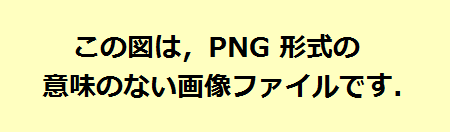
\includegraphics{fig1.png}
  \caption{意味のないPNG形式の図}
  \label{fig:png}
\end{figure}
\begin{figure}
  \centering
  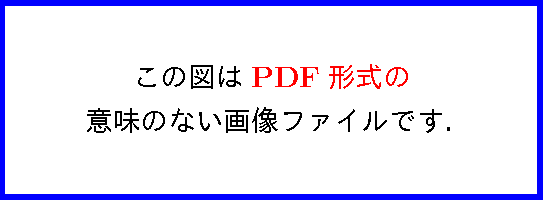
\includegraphics{fig2.pdf}
  \caption{意味のないPDF形式の図}
  \label{fig:pdf}
\end{figure}
これでこの文書中には図\ref{fig:png}と
図\ref{fig:pdf}が挿入される.
\end{document}
\end{lstlisting}

% さて,画像挿入の際には,タイプセットを行う前に,
% 画像がどれくらいのサイズであるかの情報(BoundingBox)を収めた
% ファイルを作成しなければならない.コマンドプロンプトで
% \begin{lstlisting}
% > extractbb fig1.png
% > extractbb fig2.pdf
% \end{lstlisting}
% を実行すると,
% BoundingBoxが格納された\FNAME{fig1.xbb},~\FNAME{fig2.xbb}が生成される.
% その後のタイプセットはいつも通りである.
これをいつも通りの方法でタイプセットすれば,画像が含まれた PDF ファイルが生成される%
\footnote{%
  現在の\TeX Live では\verb|extractbb|は自動実行される.
}.
\begin{lstlisting}
> uplatex grapheg.tex
> uplatex grapheg.tex
> dvipdfmx grapheg.dvi
\end{lstlisting}

% \medskip

% 画像ファイルが増えるたびに\FNAME{extractbb}を実行しないといけないのは
% 面倒だ,という人は,\pLaTeX 実行時に\hskip\ltjgetparameter{xkanjiskip}%
% \texttt{-shell-escape}オプションを追加して
% \begin{lstlisting}
% > platex -shell-escape grapheg.tex
% \end{lstlisting}
% または,\FNAME{ptex2pdf}を使うなら
% \begin{lstlisting}
% > ptex2pdf -l -ot -shell-escape grapheg.tex
% \end{lstlisting}
% のようにすれば,\FNAME{extractbb}は自動で実行される.
% しかし,この\hskip\ltjgetparameter{xkanjiskip}%
% \texttt{-shell-escape}オプションは外部のプログラムを実行可能にするものなので,
% セキュリティ上の問題を引き起こすこともある\footnote{そのため,
% 標準ではいくつかの「安全だとわかっている」プログラムに限り実行が許可されている.
% \FNAME{extractbb}をそのリストに追加するには,
% \href{http://oku.edu.mie-u.ac.jp/~okumura/texwiki/}{\TeX~Wiki}中の「\TeX 入門/図表」
% を参照すること.}.
% そのため,面倒だが手動で\FNAME{extractbb}を実行することを勧める.


\subsection{図式}
数学では,
\[
  \begin{tikzcd}
    & C \ar[ld,bend right=15,"f"']
        \ar[rd,bend left=15,"g"]
        \ar[d,dashed,"{(f,g)}"] & \\
    A & A\times B \ar[l,"\pi_1"] \ar[r,"\pi_2"'] & B
  \end{tikzcd}
\]
のような図式を使う(上は直積のuniversalityを表したものである).
このような図式を記述するには\PKG{tikzcd}というパッケージを使うのが便利である.
詳しい使い方は,
\texttt{texdoc tikzcd}
を参照して欲しい.

この図式の出力は,プリアンブルに
\begin{lstlisting}
\documentclass[uplatex,dvipdfmx]{jsarticle}
\usepackage{tikz-cd}
\end{lstlisting}
と入力することで\PKG{tikzcd}を読み込んだ上で,
\begin{lstlisting}
\[
  \begin{tikzcd}
    & C \ar[ld,bend right=15,"f"']
        \ar[rd,bend left=15,"g"]
        \ar[d,dashed,"{(f,g)}"] & \\
    A & A\times B \ar[l,"\pi_1"] \ar[r,"\pi_2"'] & B
  \end{tikzcd}
\]
\end{lstlisting}
というソースで行った.

図式中に登場する$A$,~$B$などのオブジェクトは,
\ENV{tabular},~\ENV{array}環境などのように表の形で入力する.
\texttt{\&}が列の区切り,\verb+\\+が行の区切りである.
図中$C$は第1行第1列……のように見えるが,第2行第2列の$A\times B$の真上にくるように
タイプセットしたいので,ソース中では\emph{第1行第2列}の位置に指定する.

\cs{ar}(または\cs{arrow})で始まるのが図式中の矢印である.
矢印の終点やラベルの内容は,\cs{ar}の(角かっっこ)引数として指定する.
\begin{itemize}
\item 矢印の終点は,始点からの相対位置で指定する.例えば,\verb+\ar[llu]+ならば,
  相対的に2つ左(\textbf{l}eft),1つ上(\textbf{u}p)のオブジェクトに向かって矢印を書くことになる.
\item 矢印には上下にラベルを付けられる.
  ラベルは二重引用符\verb+" "+で囲む.
  追加の指定をしない場合は進行方向向かって左側に付くが,右側に付けたい場合はアポストロフィー\verb+'+を二重引用符の直後に付ける.
  上のソース中の\verb+\ar[l,"\pi_1"]+と\verb+\ar[r,"\pi_2"']+を比較して欲しい.
  注意点として,ラベルの中身がコンマを含む場合は,ラベルを波括弧で囲う必要がある.
\item 線種の指定もできる.
  通常の矢の他に可換図式で良く使うものとしては
  \[
    \begin{tikzcd}
      A \ar[r,equal]
      & B \ar[r,dashed]
      & C \ar[r,twoheadrightarrow]
      & D \ar[r,rightarrowtail] & E
    \end{tikzcd}
  \]
  などがあるが,これらは
\begin{lstlisting}
\[
  \begin{tikzcd}
    A \ar[r,equal]
    & B \ar[r,dashed]
    & C \ar[r,twoheadrightarrow]
    & D \ar[r,rightarrowtail] & E
  \end{tikzcd}
\]
\end{lstlisting}
  によって入力できる.
\item 矢印を少し曲げたい場合には,\texttt{bend left}, \texttt{bend right}でそれぞれ進行方向左側・右側に曲がる.
  オプションの値として数値を指定することで,曲がり具合を調整できる(小さい方がより真っ直ぐに近い).
\end{itemize}

\paragraph{}
次の図式(five lemmaの図)をタイプセットせよ.
\[
  \begin{tikzcd}
    A \ar[r,"f"] \ar[d,"\alpha"'] & B \ar[r,"g"] \ar[d,"\beta"'] & C \ar[r,"h"] \ar[d,"\gamma"'] & D \ar[r,"i"] \ar[d,"\delta"'] & E \ar[d,"\epsilon"'] \\
    A' \ar[r,"f'"'] & B' \ar[r,"g'"'] & C' \ar[r,"h'"'] & D' \ar[r,"i'"'] & E'
    \end{tikzcd}
\]

\paragraph{}
次の各図式をタイプセットせよ.
\begin{align*}
  \begin{tikzcd}[ampersand replacement=\&]
    1 \ar[r,"a"] \ar[rd,"z"'] \& A \ar[r,"f"] \ar[d,dashed,"x"] \& A \ar[d,dashed,"x"] \\
    \& N \ar[r,"s"'] \& N
  \end{tikzcd}
  &&
  \begin{tikzcd}[ampersand replacement=\&]
    X \ar[r,bend left=20,"f"] \ar[r,bend right=20,"g"']
    \& Y \ar[r,twoheadrightarrow,"q"] \ar[rd,"e"']
    \& Q' \ar[d,dashed,"e"] \\
    \& \& A
  \end{tikzcd}
\end{align*}

\paragraph{}
次の図式をタイプセットせよ.
\[
  \begin{tikzcd}
    &&&& Y' \ar[dd,"e"'] \ar[r] & Y \ar[dd,"p"] \\
    Z'\times_C D \ar[d,"z"'] \ar[r] \ar[rd,phantom,"\text{p.b.}" description] % p.b. をもう少し小さくしたいが…
    & Z' \ar[r] \ar[d,"c"']
    & Y' \ar[r,twoheadrightarrow] \ar[rru,equal,bend left=15]
    & e(Y') \ar[d,"m"] \ar[rd,hookrightarrow] & & \\
    D \ar[r] \ar[d,"p"']
    & C \ar[rr,twoheadrightarrow] &
    & B' \ar[r,twoheadrightarrow]
    & X' \ar[r] \ar[d,"f'"']
    & X \ar[d,"f"] \\
    B \ar[rrrr,twoheadrightarrow] & & &
    & A' \ar[r,twoheadrightarrow] & A
  \end{tikzcd}
\]

% 複雑な配置を行いたい場合は,\PKG{tikzcd}を使うよりも,大本となる図形描画パッケージTikZを直接使った方がいいかもしれない.

\subsection{数式クラス}

TODO: 書きたい

「数式組版」を紹介する?

\newpage

\subsection{難しい小ネタ}

\paragraph{}
以下の内容のソースファイルを\FNAME{twice.tex}として保存し,タイプセットせよ.
そして,なぜそのような出力結果が得られるのかを説明せよ.
\begin{lstlisting}[xleftmargin=3\zw, numbers=left, numberstyle=\tiny]
\let\Enddoc\fi
\iffalse

あいうえお

\Enddoc
\documentclass{jsarticle}
\begin{document}

かきくけこ

\def\Enddoc{\end{document}}
\makeatletter
\let\@@let=\let
\def\let#\char35#1#\char35#2\iffalse{%
  \global\@@let\let\@@let}
\@@input \jobname.tex
\end{lstlisting}
%%% 答え:
%%% 1. \iffalse .. \fi は読み飛ばされるので
%%%    2--6 行目は読み飛ばされる.よって,
%%%    > \documentclass{jsarticle}
%%%    > \begin{document}
%%%    >
%%%    > かきくけこ
%%%    >
%%%    > \def\Enddoc{\end{document}}
%%%    > \makeatletter
%%%    > \let\@@let=\let
%%%    > \def\let#\char35#1#\char35#2\iffalse{%
%%%    >   \global\@@let\let\@@let}
%%%    が順に実行される.
%%% 2. さて,この後,17 行目の \@@input で,twice.tex 自身が
%%%    もう一回読み直されることになる.
%%% 3. このとき,1--2 行目は 15, 16 行目の \let の再定義により
%%%    > \global\@@let\let\@@let
%%%    (つまり,再定義された \let を下に戻す)処理に置き換わる.
%%% 4. その後,3, 4, 5 行目と順に進み,6 行目の \Enddoc に到達するが,
%%%    1 回目の読み込み時に 12 行目において \Enddoc は
%%%    > \end{document}
%%%    という内容になっている.
%%% 5. 以上より,今度は 6 行目でタイプセット処理が終わる.
%%%
%%% 結果として,タイプセット全体では次のソースを処理しているのと
%%% ほとんど変わらない状況となる:
%%%    > \documentclass{jsarticle}
%%%    > \begin{document}
%%%    >
%%%    > かきくけこ
%%%    >
%%%    >
%%%    > あいうえお
%%%    >
%%%    > \end{document}

\paragraph{}
\<\emph{(幻の``\texttt{This can't happen}''を拝もう)}


\TeX\ - \LaTeX\ Stack Exchange中の
\href{http://tex.stackexchange.com/questions/31517/shortest-code-causing-emergency-stop-error}%
{Shortest code causing ``Emergency stop.''~error}という投稿によれば,
以下の1行からなる\TeX ソース:
\begin{lstlisting}[numbers=left,numberstyle=\tiny,xleftmargin=3\zw, literate={\$}{\#}1]
\halign{$&&$\cr\multispan{300}\cr}
\end{lstlisting}
が``\texttt{This can't happen}''を引き起こすそうだが,残念ながら
\begin{lstlisting}[numbers=left,numberstyle=\tiny,xleftmargin=3\zw, literate={\$}{\#}1]
\documentclass{article}
\begin{document}
\halign{$&&$\cr\multispan{300}\cr}
\end{document}
\end{lstlisting}
を筆者の環境の\pLaTeX でタイプセットしてもそうはならなかった.

\medskip
しかし,「\pTeX・\pLaTeX はバグが少ない,やったね!」とは決して言えない.
\pTeX の日本語対応には不完全なところがまだ残っており,
短い\TeX ソース(本質的には1行)で,\pLaTeX でタイプセットすると
\begin{lstlisting}
! This can't happen (disc4).
\end{lstlisting}
というエラーを発生させるものが存在する.
さて,誰か自力でそれを発見できないだろうか?

%%%%% これが解ける人は「もう引き返せない」人でしょう.
%%%%% TA 用に答えも載せておきます(以下の 3 行):
%%% \documentclass{jsarticle}
%%% \begin{document}
%%% \discretionary{}{}{あ}\unskip

\end{document}
